\section{Boundaries of Operations Management}

To contextualize operations management within an organization, it is necessary to understand its boundaries. Most organization rely upon a large collection of supporting functions that exist in large part to ensure the success of the operations area \parencite{mcadamRoleLeanInterface2016}.

Typical support services include areas such as supply chain management, contract management, sales management, marketing, customer service, facilities management, HR management, financial management, IT Management (for operations that are not IT services), security services, logistic services and many others.

Many of these services are themselves providing key inputs into the transformational engine that is operations. For example, supply chain management is responsible for ensuring that the operations receive the necessary parts and raw materials to produce the quantity of goods/services that the operations team is planning on producing. In order for this to happen effectively there are multiple feedback loops involved. Operations needs to provide to marketing their minimum and maximum production rates, marketing needs to work with the sales teams to determine the expected order velocity for the organization. Marketing then needs to provide this information back to operations. Operations will then inform the supply chain management team of their demand and schedule to meet marking goals (see fig \ref{fig:chain})

\begin{minipage}{\linewidth}
  \makebox[\linewidth]{ % to center image}
    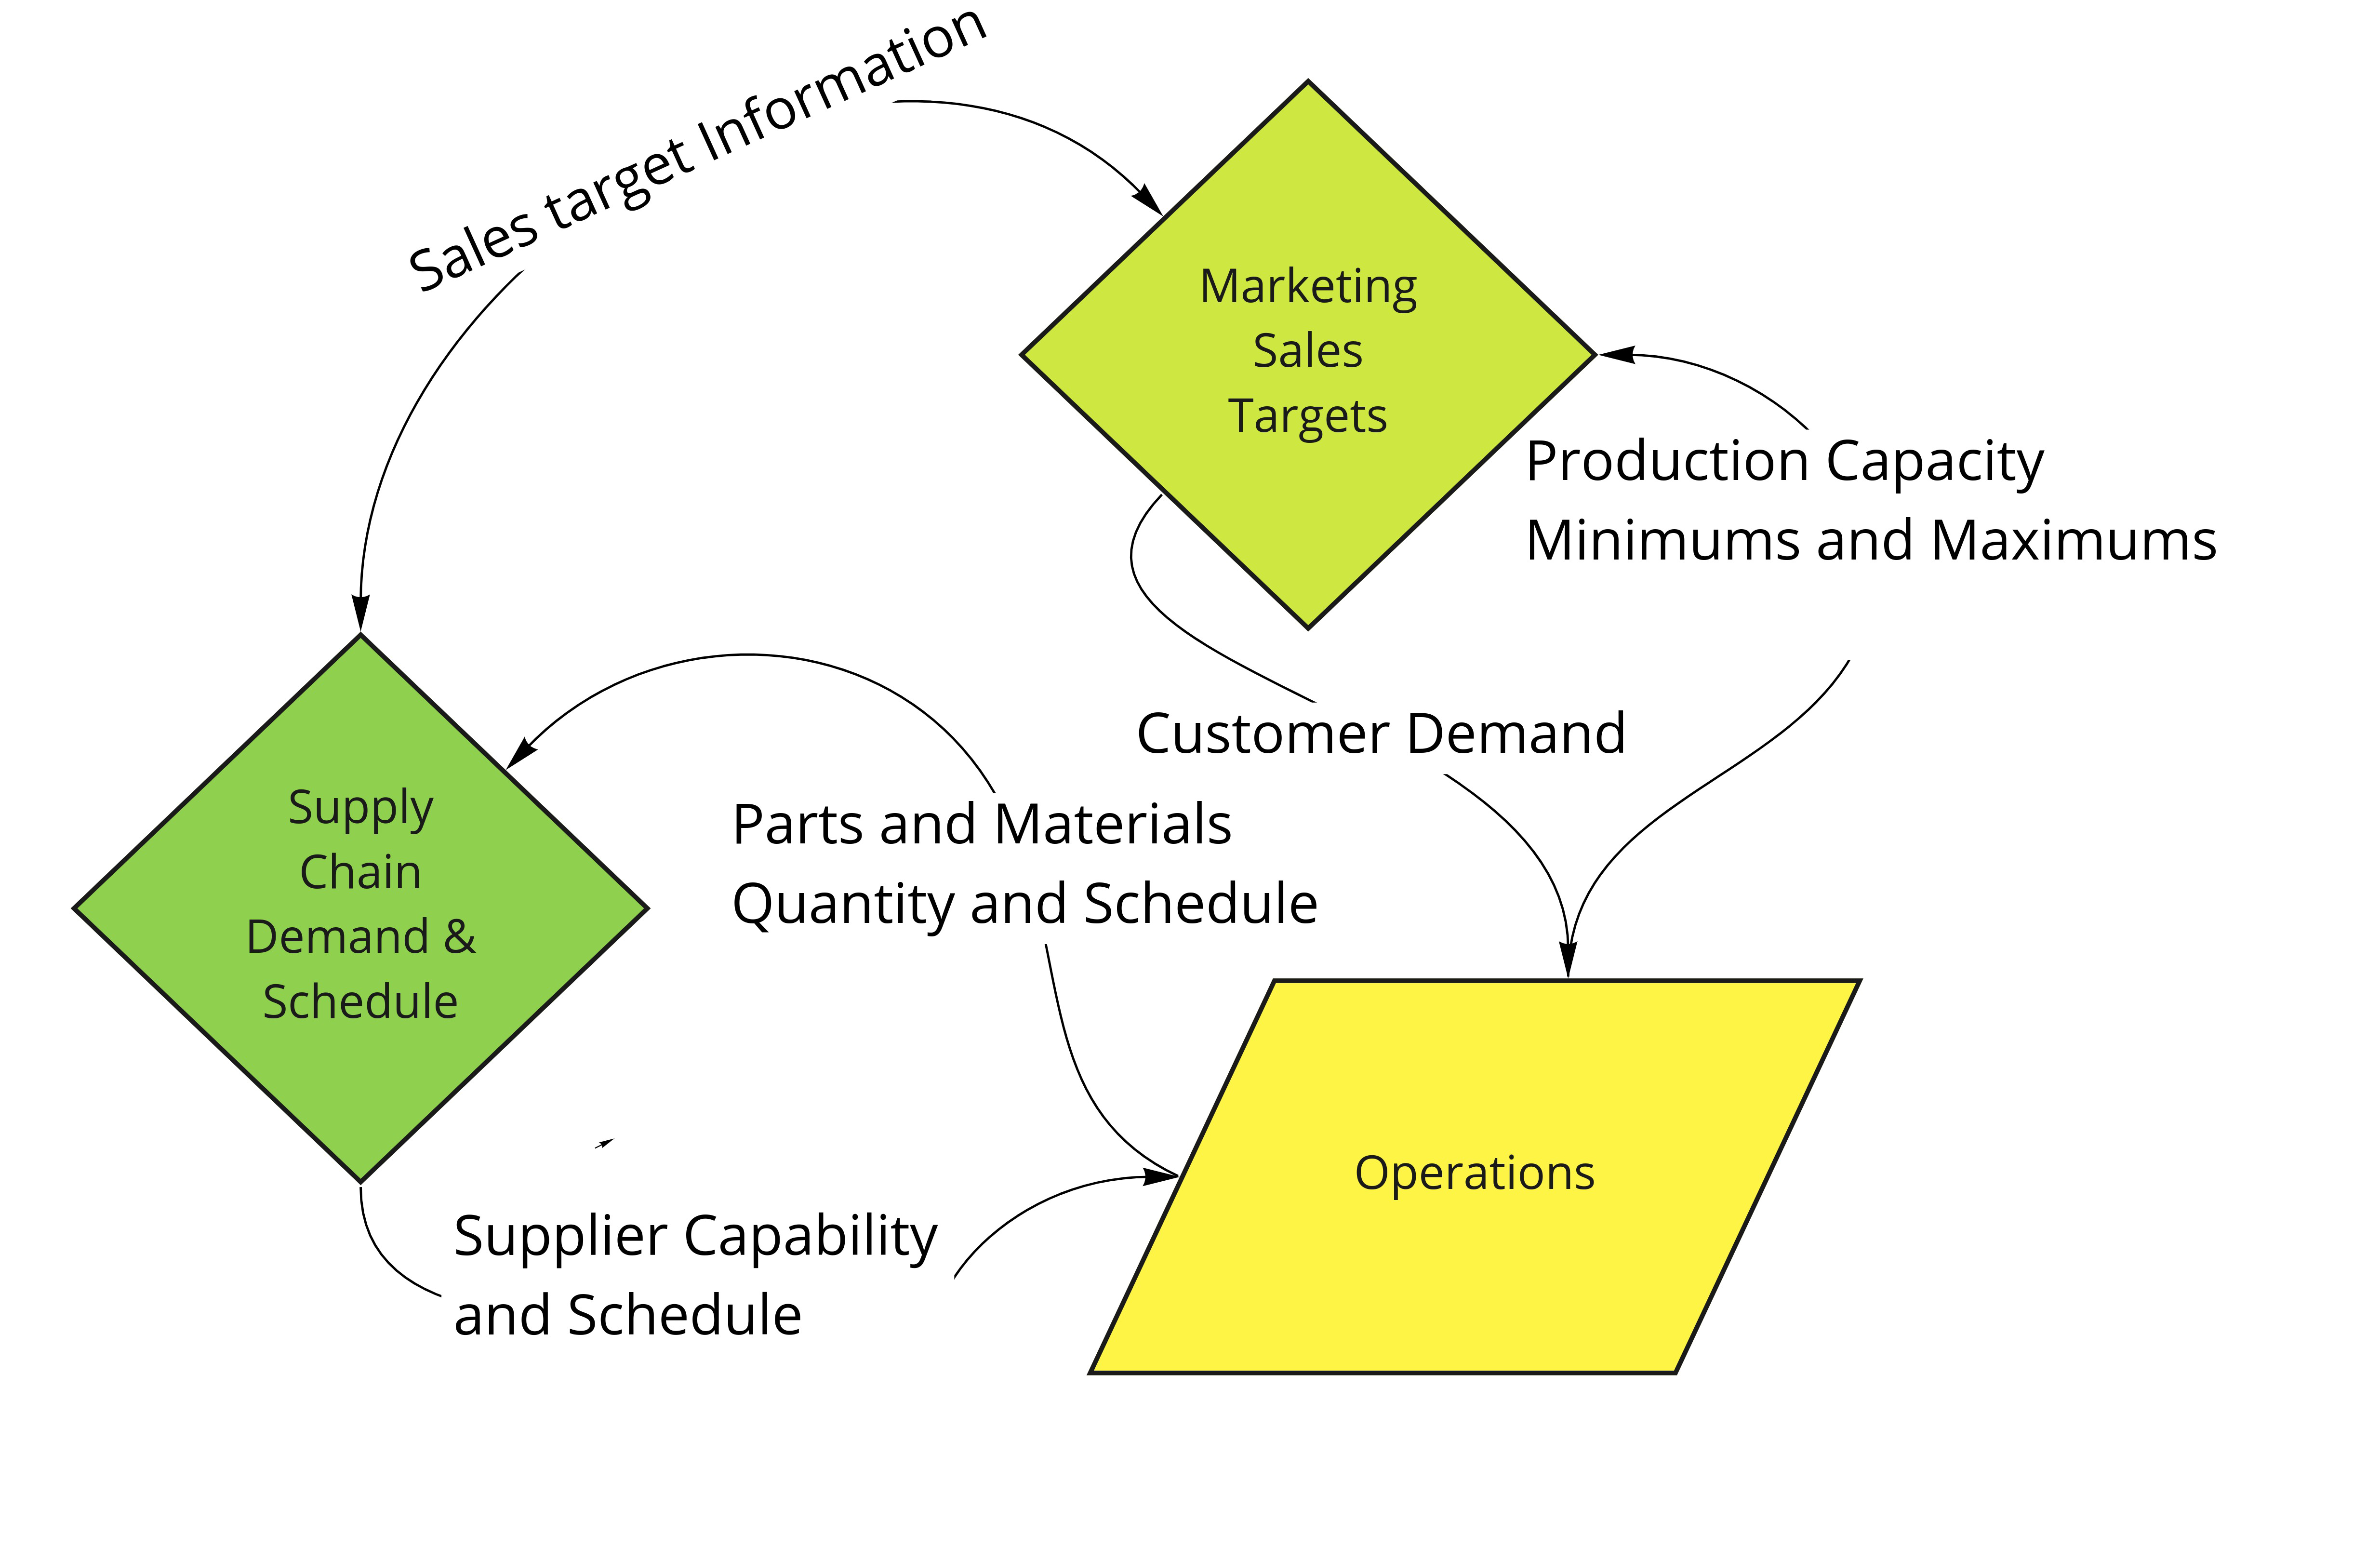
\includegraphics[width=6in]{img/supplychain}}
    \captionof{figure}{Operations/Supply Chain/Marketing}
    \label{fig:chain}
\end{minipage}

Of course, the interactions are more complex than this. Marketing, for example, is also responsible for understanding the customers' wants and needs and making recommendations to product design engineers. These engineering teams then will work with production engineers who are part of operations to provide suggestions for how to improve the resulting product or service. This is an important source of product innovation and directly correlates to long-term organizational succes \parencite{dattomaDeterminantsTechnologicalInnovation2020}.

Similarly, on the back-end of operations, order fulfillment, billing and receiving, and customer service are departments that are frequently outside the boundaries of operations. While operations managers are rightly concerned about these functions, they are support functions to the transformational process that is the heart of operations.

Shipping and logistical support to provide the goods and services to the end-user of the product can itself be a significant and complex endeavor. It is not uncommon for products to be shipped in an incompleted state between intermediate operations. For example, many consumer level electrical applicances see final packaging happen in a specific geographic location due to the different electrical system standards in various countries. By waiting until the last moment to package the power system, the operations team does not have to worry about forking production counts for each unique powergrid. Rather, production can consider global, or at least regional, production as a whole, and thus lessen complexity by utilizing just-in-time assembly. Similarly, feedback from sales and marketing, can help shape the mix of products produced in order to provide maximal value to the customer base \parencite{tavakkoli-moghaddamMemeticAlgorithmMulticriteria2006}.
